\documentclass[notitlepage]{article}
\usepackage[left=1in, right=1in, top=1in, bottom=1in]{geometry}
\usepackage{graphicx}
\usepackage{titling}
\usepackage{lipsum}
\usepackage{amsmath,amssymb}
\usepackage{amscd, amsthm, mathrsfs,amsfonts}
\usepackage{svg}
\usepackage{float}
\usepackage{gensymb}
\newtheorem{theorem}{Theorem}
\usepackage[toc,page]{appendix}
\usepackage{ mathrsfs }
\usepackage{graphicx}

\newtheorem{definition}{Definition}[section]

\pretitle{\begin{center}\Huge\bfseries}
\posttitle{\par\end{center}\vskip 0.5em}
\preauthor{\begin{center}\Large\ttfamily}
\postauthor{\end{center}}
\predate{\par\large\centering}
\postdate{\par}

\title{Quantized directional freedom or the Lightlane Conjecture}
\author{Jens Bjørlo Tandstad}
\date{\today}
\begin{document}

\maketitle
\thispagestyle{empty}
\begin{abstract}

Gerard t'Hooft has in the Cellular Automaton Interpretation of Quantum Mechanics \cite{hooft2014cellular} indicated that Cellular Automatons are viable as a foundation for Quantum Mechanics. In this paper we attempt to study one implication this would have for astrophysics, if it is true, "The Lightlane Conjecture". The conjecture applies Construction Theory by David Deutch and Chiara Moretti \cite{DeutchMoretti}, \cite{MorettiVedral} as a theoretical foundation, using it to analyze the effects of constraints that apply to a broad class of Cellular Automata. Cellular Automatons are able to circumvent Weyl's tile argument, if they carry with it a "program" of information corresponding to the precision of its directional propagation options through space. We show that the length of this information program in the limit approaches classical physics, but not when the program length is finite.
\end{abstract}

\section{Introduction}
Constructor Theory  is a framework for scientific inquiry suggested by David Deutch and Chiara Marletto \cite{DeutchMoretti}, \cite{MorettiVedral}. The approach is suitable to make predictions about any kind of discretely functioning machinery. In stead of making a theory fit experimental data, Constructor theory is concerned with constraining the space of possible and impossible universes that can arise from axioms, and the aggregate effects of such constraints. Although Constructor Theory presents a theoretical foundation for this type of reasoning, it has been used before. For example, it is possible to estimate the error term of the calculation of floating point number representations in computers, by seeing how the constraints on the mechanics for division actually happen. Another example of a similar type of reasoning is Hawking radiation, combining phenomena at the quantum level (virtual particles) with gravity, indicating that black holes must evaporate as they attract antimatter from virtual particles. Constructor theory generalizes this notion of using constraints to limit the range of possible outcomes into information theory.

Constructor Theory is designed as a framework to make predictions about physical reality based on constraints formulated using information theory. The study of information has been suggested as a possible foundation of Quantum Mechanics by several notable physicists over the last century. There are many points of contact, including the Pauli exclusion principle, seemingly excluding the possibility for fermions to have the same exact quantum values. One way to think about this is that if they had the same values, they would be the same particle. This is very counterintuitive to a classical mind. However, it has long been accepted in set theory that existence is defined through something being identical to itself, $\exists x(x = x)$. From a philsophical standpoint, it's possible that the Pauli Exclusion principle is related. John Wheeler coined the phrase "it from bit", suggesting that reality is arising from information relationships, and that we as observers are simply features of this information relationship, perceiving the structure from within. Edward Fredkind suggested in his paper "Calculating space", that the universe and therefore reality is simply the evolution of an information system. 

It is quite obvious from Heisenbergs matrix formulation, that Quantum mechanics is related to information theory. Crucially, the notion of discrete quantum states is philosophically related to the question of whether spacetime is quantized. If so, information must be able to move across this quantized substrate. It turns out that the problem of information propagation through quantized space is very deep. Hermann Weyl's argues in his "Tile argument" that a distance metric cannot be defined for a quantized grid, and therefore space cannot be discrete. Tobias Fritz of the Perimeter institute have attempted to convert Weyls tile argument into a  \cite{FritzNoGo} no-go theory for all digital-physics theories. However, Jean Paul Van Bendegem at Stanford have posed a strong counter-argument \cite{stanford-geometry-finitism}. It's possible that the difficulty of reconciling quantum mechanics with general relativity is not a technical issue, but a deeper one involving the philosophy of science as well as information theory.

Notable figures have investigated information theoretic foundations for Quantum Mechanics. These theories all accept Quantum Mechanics as valid, but are unsatisfied with the Copenhagen Interpretation which avoids any pretense that something can be hiding at an even deeper level. Because QM is well proven, such candidates for foundations must support the emergence of both quantum mechanics and general relativity. A recent work investigating such a connection is Nobel Laureate Gerard t'Hooft Cellular Automaton Interpretation of Quantum Mechanics  \cite{hooft2014cellular}. In this work, T'Hooft constructs a classical "cog-like" device using Cellular Automatons (CAs). CAs are a deterministic, self-preserving information relationships which gains persistence through evolving through discrete steps, and returning to a previous configuration. Because it is deterministic it then will inevitably loop. Using the constraints that follow from such constructs, t'Hoofts shows in his under-appreciated work that CAs and their interactions are sufficient as a foundation for Quantum Mechanics. It's clear that such discrete information mechanisms also require an information substrate on which they exist and move around, which actualizes Weyl's tile argument and the critique of it.

Meanwhile, Stephen Wolfram has taken a different but related approach. In a strikingly original way, the Wolfram Physics Project \cite{Wolfram2020} has dug into the complexity generated by simple substitution rules. This can be understood as possible relationships between a graph and a rule, and creates relationships through applying the same rule over and over again onto extremely parsimonious initial conditions. In the Wolfram Physics project, Stephen Wolfram and his team have studied such evolution rules extensively. They show, that some of these rules knit lattice-like graphs over time. Studying the resulting graphs, their team has been able to find analogs of many phenomena both from Quantum Mechanics and General Relativity. For example, the graph itself can be seen as (locally flat) Hilbert space. Through interpreting the evolution of causal edges on the graph, features such as the Feynman path integral, Ricci tensor and intuitive explanation for heat, quantum indeterminance emerge. Also, these rules support - at least in theory - features of the graph that self interact in specific ways. It remains to be seen if the Wolfram Physics project, Constructor Theory and t'Hoofts Cellular automaton interpretation converge, but if they do - there is hope that a theory of everything can be found in the study of information relationships and their evolution. Although the definition is not agreed upon, approaches that begin with space being quantized at the Planck Scale (or below) can be collectively called Digital Physics theories.

\section{Falsification of Digital Physics theories}
So far, Digital Physics has not made any testable predictions. This is to be expected, as the theories begin - not with observations - but through grappling with the discreteness of Quantum Mechanics. Given the risks and the low probability of making any headway, such topics are usually avoided entirely, and left a small minority interested in the foundations of Quantum Mechanics, such as Gerard t'Hooft, David Deutch, Chiara Moretti, Stephen Wolfram etc. Notably, both John Wheeler, Richard Feynman, Bryce DeWitt, Roger Penrose, John Von Neumann, Hugh Everett and many others has been investigating digital representations of life. The prevailing assumption seems to be that starting from intuition and working upwards will never result in predictions that can be tested empirically. One could say there is an \textbf{assumption of metaphysical untestability}. 

In this paper I  argue there is away to test certain interpretations of Quantum Mechanics. Through Constructor Theory, an axiomatic metaphysics can be converted into real physics, if the metaphysics explicitly requires or precludes certain types of behavior, which are subsequently empirically falsified. For example, if the metaphysical axiom specifies that the universe is a grid, and everything that exists is simply information on that grid - then as a consequence of that, nothing can be between two cells on that grid. Such an axiom predicts that there must be a minimum distance in the universe. In fact, the rules of propagation over a crystalline substrate has been studied in chemistry for over a century.  

Suppose that movement in space is subject to Weyl constraints on their movement. The suspicion is warranted, because in Quantum Mechanics have discovered a theoretical minimum distance called the Planck Length.  The theory implies that further subdivision of this length $ \ell_P $ is meaningless within the theory itself. Because Quantum Theory is essentially correct, we must take such hints about the nature of the universe seriously. 

The Lightlane Conjecture is concerned with applying constraints on what is possible, and realizing this into a a testable prediction. As the remainder of this paper will show, by adding additional axioms from the theory of Cellular Automata, identifying constraints associated with quantized space-time, and using the approach from Constructor Theory about possible and impossible tasks, it is possible to make predictions about starlight.

\section{The pesky problem of free directional movement}
We begin by imagining the universe as a two dimensional grid, and a photon is a local information feature existing on that grid. Suppose the photon consist of 5 disturbances (or excitations), such as in \ref{fig:glider}. Each disturbance is binary, and confined to a cell on the grid. Because the value cannot be in-between cells, the grid constrains information pattern by requiring it to be aligned to the grid. We are interested in the constrains that affect this patterns ability to move through the grid. 

Let us name this pattern the Glider make sure we understand it completely.

\begin{figure}[!ht]
  \centering
 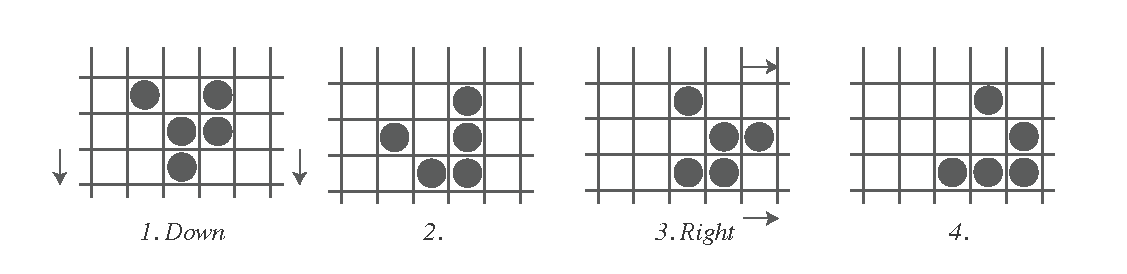
\includegraphics[width=0.9\textwidth, trim={0cm 0cm 0cm 0cm},clip]{Illustrations/Glider.pdf}
  \caption{The glider pattern in the "Game of Life" Cellular Automata is a periodic map.  )  }
      \label{fig:glider}
\end{figure}

The pattern evolve according to the following evolution rules:

\begin{enumerate}
\item Any live cell with fewer than two live neighbours dies, as if by underpopulation.
\item Any live cell with two or three live neighbours lives on to the next generation.
\item Any live cell with more than three live neighbours dies, as if by overpopulation.
\item  Any dead cell with exactly three live neighbours becomes a live cell, as if by reproduction.
\end{enumerate}

Each time it loops, it moves one step to the right and one step down (indicated by the little arrows. It able to move in 4 distinct directions, depending on its initial orientation, of which only four are possible. The rule is always the same and is applied to each cell, while only being aware of the neighbouring cells. This locality constraint is what makes this a local theory, and CAs which have this constraint is called \textbf{totalistic} Cellular Autoamtons (TCA).

The Glider in Fig \ref{fig:glider} is is perhaps the most famous TCA rule, and is operating on a rectangular grid in $\mathbb{R}^2$. Due to the incredible variety of rules and grids, there will be analogues for the glider in higher dimensions and other grids, such as for example tetrahedral $\mathbb{R}^3$ and tesseractic in $\mathbb{R}^4$ etc. The grid can also be the result of fractal evolution. The Wolfram Physics \cite{wolfram2020} project provides a rich perspective into the possible evolution of such graphs. For our purposes, we only require that the grid is locally flat and with a well defined neighbourhood. This allows us to study TCAs operating on this grid, and map their operational constraints through Constructor Theory. 

\subsection{Defintions}
We will use the Glider pattern to introduce some new concepts. Let us coin the term \textbf{Effective Directional Information (EDI)}, which is an integer and is the number of different directions that a pattern can move. The actual trajectory of the Glider is constrained to one of these four, and which one is encoded in the initial configuration in the first frame. Because the glider can move in 4 directions, it's EDI number is 4, or $2^2$. We have:

\begin{definition}
\textbf{Effective Directional Information (EDI)}: An integer specifying the number of distinct propagation paths that a Cellular Automaton can take, including it's initial orientation options. 
\end{definition}

\begin{definition}
\textbf{\textit{Bitlength} \textbf{(b)}}: The EDI of a cellular automaton expressed as the smallest power of two, that is higher than the EDI.
\begin{equation}
2^{b-1} < EDI < 2^b  \quad b \in \mathbb{Z}
\end{equation} 
\end{definition}

Throughout this paper, we will be using the bitlength $b$ in place of the EDI, the reason being that the binary encoding is the most efficient form of serialization. By using $2^b$ in place of EDI we can be sure that there is no other, more compact way of storing that information. If $c = 1$, i.e one tile per unit of time, it follows that:

\begin{equation}
|\vec{v}|_M \leq \frac{T_P}{\Omega},	\quad \Omega \in \mathbb{Z}^+
\end{equation} 

This also implies that if a CA is not wasting any ops by moving backwards, then it must be moving at the highest possible speed, i.e the speed of light.

In the Appendix, there is also a list of some other definitions and an example of applying these to the Glider, see Appendix A.

\section{Photonic TCAs and the Distance Metric}
The TCA we will present as a model for a photon must be able to move at the speed of light. We use natural units $c =1$ indicating a movement of one Planck length $L_P$ per Planck time $T_P$. We use Manhattan distance because so far, our TCAs are operating on a regular square grid. The theory of Weyl groups generalize this concept of adjacency and distance by stepwise movement through adjacent cells into all kinds of mathematical structures. As a result, there exists a corresponding distance metric for all regular crystalline substrates, the Manhattan distance is simply the one associated with the square lattice.

This is not without its problems. It introduces anisotropy to the propagation of energy and mass, the problem is most pronounced for photons because they are known to move at the maximal speed allowable. This has some very deep implications, because the euclidian metric is the one which hold on the macroscopic scale. Tobias Fritz in  \cite{FritzNoGo} has taken advantage of this conflict. He argues that the problem of a viable transition between fundamentally anisotropic Manhattan Distance and the macrosopic isotropic Euclidian distance metric can be turned into a No-Go theorem of digital physics, suggesting that all theories that quantize space has this problem. This rules out the Cellular Automaton interpretation, because it cannot possibly implement the continuous assumptions of light propagation. However, it has been suggested that a way around the No-Go theorem is use use aperiodic Penrose tiling or triangular/tetrahedral tiles. For more information, visit Jean Paul Van Bendegems excellent exposition in the Stanford Encyclopedia \cite{stanford-geometry-finitism}. A final, more exotic explanation is emergent, i.e it is a macroscopic phenomena related to how we time and movement is. After all, if \textbf{action} is constrained to move along Manhattan geodesics, and the time required to do so is the same regardless of the path, the Euclidian distance metric does not actually exist on the Planck scale at all. If it does exist, the No-Go theorem could hold and could falsify a the broad class of digital physics theories, such as the Cellular Automaton Interpretation.

Happily, for the purposes of this paper, we don't need to invoke this level of detail. The important bit is that that Cellular Automatons obey constraints on shifting it's information through adjacent cells only. We will be using the square lattice, for which the Manhattan distance is also the Weyl Distance metric, but the results are generalizable to other crystals.

\subsection{Serpentine class TCA - A workaround for the Weyl constraints}
We will now introduce a more complex Cellular Automaton with more capabilities than the Glider. The Serpentine is an example of a TCA, and its abilities and limitations are important as a mental model for the Lightlane Conjecture. The Serpentine Class of TCAs are a subset of all possible Cellular Autmatons, characterised by:

\begin{enumerate}
\item Permanence : Never disappear when left alone.
\item Conservation : Can only interact in ways that do not destroy, only exchange information.
\item Movement : Able to propagate
\item Locality : Interactions are local (neighbouring cells only)
\end{enumerate}

\begin{figure}[!ht]
  \centering
 \includegraphics[width=0.9\textwidth, trim={0cm 0cm 0cm 0cm},clip]{Illustrations/Fig1Serpentine.pdf}
  \caption{M5 Serpentine : Example of Serpentine Class TCA}
      \label{fig:serpentine}
\end{figure}

The structure presented in \ref{fig:serpentine} is inspired by the Glider and the Universal Turing Machine. \cite{turingMachine}. It consists of a tape containing instructions about whether to move up, down, left or right. A 3D version with 6 instructions is analogous and has been built as well with a surprisingly short program. The body of the Serpentine consist of the trunk lane (black), and the upstream lane (grey). The Serpentine also have a tail and head, which requires a little more explanation. On the tail of the trunk operates a Constructor mechanism called \textbf{"The gobbler"}, named because it gobbles up the trunk. It's defined as a structure acting according to the same rules as the rest of the Serpentine, which is able to perform the \textbf{gobble task.} Whenever it takes another bite of the trunk, it passes the instruction into the \textbf{upstream lane}. The upstream lane acts as a queue, passing the instructions  up on the outside of the trunk toward the \textbf{head}. When an instruction reaches the head, the instruction is laid down in front of the trunk, becoming part of the trunk.

The program executing this behaviour is remarkably simple. The class is characterized by executing a tape-like set of instructions which determine it's path of propagation over some grid. It is not constrained to the square grid, and I have successfully created an implementation operating in cubic space.  It's likely that a triangular and tetrahedral versions are also possible, but this so far proven difficult to visualize. The TCA certainly does not have all properties of the photon. Think of it as an intuitive model constructed to execute the desired task of arbitrary precision propagation. The encoding of the instructions is linear, so that the footprint $F$, i.e the space occupied by the TCA is equal to the length of both lanes, multipied by the size of each symbol, plus a constant which denote the size of the Gobbler and Head mechanism at the ends. 

\begin{equation}
F = G + IS + H
\end{equation}

Where $G$ is the footprint of the Gobbler, $I$ is the length of the tape $S$ is the footprint of each symbol on the tape, and $H$ is the size of the head. Both $G$, $S$ and $H$ remain undefined for this class. The Serpentine is \textbf{implementation agnostic}, but it remains \textbf{totalistic}, because the individual tasks performed by the four parts (Gobbler, Head, Trunk, Lane) are all only reliant on the state of neighbouring cells. 

\subsection{From discrete to continuous}
The Serpentine is an example of a \textbf{class of discrete information structures} which can approach continuum performance by extending its onboard information. It is an interesting class of objects, because such a class is required to bridge the discreteness of Quantum Mechanics with General Relativity, under the assumptions that the Cellular Automaton Interpretation holds.

It is clear that the propagation direction through space is given by the number of forward instructions relative to sideways instructions on the tape. A short trunk implies an equally short lane, and that implies a lower number of realizable integer fractions corresponding to possible directions. It follows that the Serpentine TCA can be made to move in \textbf{any} direction, provided that we add more instructions to the tape. In the naive limit, the Serpentine tape must be infinitely long in order to support infinite precision. Throughout this paper, the M5 Serpentine will represent the entire Serpentine class of TCAs, but also serve as a crude model for the photon. This allows us to reproduce a minimum of the known features of the photon itself:

\begin{itemize}
\item Move at speed of light $c = 1, $  or $1\ell_P $ per Planck time $T_P$, using Manhattan Distance metrics.
\item Be able to have arbitrary directional precision due to onboard localized information
\item Locality (be a totalistic cellular automaton)
\end{itemize} 

All members of this class share the property of constrained directional freedom, resulting from the Weyl constraints on the propagation surface. However, they can counteract the limit by adding more information.
This is clearly a very crude template for the photon, and remains in violation of established photonics. However, this does not imply that all Serpentine Class TCA are in violation. 


\subsection{TCAs and the wave-Particle duality}
However, one problem appears to apply to the entire Serpentine class of TCAs. The Serpentine does not offer an intuition to understand the wave-particle duality. If a photon is a TCA, it is fundamentally particle like. However, it is not point-like, but it is localized with defined volume in the space. Consequently, the particle does not spread out equally in all direction. The easy way out is to build on the work of Gerard t'Hooft,  has shown in The Cellular Automaton Interpretation of Quantum Mechanics \cite{hooft2014cellular} that TCAs are viable foundations for quantum mechanics. We can then simply state that the Serpentine class of TCAs is a subclass of the TCAs used by t'Hooft. This brings the conjecture in line with Quantum Mechanics. 

Much like for Quantum Mechanics itself, this does not immediately give an agreeable intuition wave-particle duality. It seems that the only applicable intuition is that wave-like behaviour could be the result of uncertainty about the actual information hidden inside the Serpentine TCA. This uncertainty about which way the photon is moving naturally realizes a probability density which expands at the speed of light over time. To believe photons contain hidden information about their actual path, is essentially Einstein position, opposing Niels Bohrs view and formalized in the Einstein Podolsy Rosen paradox entanglement experiment. This was a major development of Quantum Mechanics, and the history is well explained by Arthur Fine, see \cite{sep-qt-epr}. However, this paradox was resolved by John Bell, through the Bell inequalities, which falsify faster than light communication between entangled quantum states. What is perhaps less known, is that the the Bell inequalities does not falsify all interpretations, such as the Many World interpretation of Quantum Mechanics. Lev Vaidman has written beautifully on this  \cite{sep-qm-manyworlds}, as well as with Kelvin J. McQueen in \cite{Many-Worlds-Interpretation}. 


\section{The simple theory of lightlanes}
We will now follow the Weyl constraints and explain how this could lead to testable predictions.

\subsection{Constraining directional precision}
As a model of a photon, it is clear that the M5 Serpentine can be made to propagate at any angle on any regular grid, at the expense of a longer tape, i.e higher EDI. The most efficient way to encode the EDI integer is in binary form. If we assume that the EDI is compressed, and that Definition 2.2 hold, how large does $b$ need to be, to allow sufficient precision to allow the photon to travel from anywhere to anywhere else sin the observable universe, with absolute precision? This question is actually a formulation of what classical physics are currently expecting photons to be able to do, based on the continuous  equations  we are using in physics. The answer depends again, on what accuracy is sufficient. We are lucky to have reached such an advanced level of Quantum Theory and cosmology to be able to answer this question: The Planck Length $\ell_P$ is the smallest distance that are meaningful in Quantum Theory. It is currently defined to be $1.61622837 \times 10^{-35} m $ , and the size of the observable universe defined to be $8.8\times10^{26} m$ across. The observable universe therefore is $5.44 \times 10^{61}$ times larger than the Planck Length. As the Serpentine TCA is confined to the information grid on which is operates, it cannot move in Euclidian geodesics, and uses Weyl Distance geodesics. In the case of the regular square grid, this allows for a simple calculation of the worst-case number of discrete steps required to traverse the observable universe with precision down to individual Planck lengths. The smallest possible angle would be exactly one step upward, and the remainder in an orthogonal direction for a total of $I$ instructions.
The minimum angle increments of propagation is given by:

\begin{equation}
\theta_{min}  = \cos(\frac{1}{I-1}), \quad I \in \mathbb{Z}
\end{equation}

For a square lattice space manifold, the worst case number of instructions on the tape before looping $\overline{I}$ must then be given by the inequality.

\begin{equation}\label{eq:universesize}
2^{b-1}< \overline{I} <= 2^b, \quad  2^b = \frac{U_L}{\ell_P} = \frac{8.8\times10^{26} }{1.61622837 \times 10^{-35}} 
\end{equation}

Solving for $b$ and rounding up gives us $b = 204$. This yields

\begin{equation}
 2^{203} < \overline{I} < 2^{204}
\end{equation} 

204 bits. Not more, not less. In order for a Serpentine class TCA to have virtually infinite directional freedom, as is ascribed to it by both  classical and quantum physics, it need no more than $b \leq 204$ to reach any point in the universe from any point, with perfect precision. This acts to place an upper bound. The lower bound, or the minimum amount of EDI that light needs to have to be able to appear as we expect is probably more interesting, and as it turns out - much more difficult and wrought with surprising twists.
We can also work this the other way, starting with a specific EDI to saying something about the pattern. Consider a photon with $2^b$ of EDI. This limits the number of possible directions the light can travel to $2^b$ options from its origin. We refer to each of these possible escape paths as \textbf{Lightlanes} represented by the vector $\vec{L}$. See figure \ref{fig:thejuul}.

\begin{figure}[!ht]
  \centering

 \includegraphics[width=0.8\textwidth, trim={0cm 0cm 0cm 0cm},clip]{Illustrations/lightlanes.pdf}
  \caption{Lightlanes with $b$ = 3 and 4. Lanes double for each increment of b. }
      \label{fig:thejuul}
\end{figure}


\subsection{Expected Photon Count equation in 2D}
To proceed, we use a thought experiment. We shall compare the classical expectation, which assumes infinite directional freedom, to the Lightlane implementation using the M5 Sepentine. Let there be a \textit{point source} of Serpentine photons, emitting randomly in all possible directions. In figure \ref{fig:thepizza}, we place a detector occupying $D$ of the circumference at distance $d$ from the light source. The expected number of photons received $\gamma_c $, equal the proportion of the detector to circumference at distance $d$. 

Let the classical \textbf{expected photon count} equation (assuming infinite directional freedom) be equal to the size of the detector $D$ as a share $\theta_D$ of the circumference at distance $d$. We emit $E $ photons from the origin, then this equation tells us the share of photons received by the detector.


\begin{equation}\label{eq:classicalPC}
\hat{\gamma_c} =  \frac{D}{2d\pi}E 
\end{equation}
We simplify this to the angle covered by the detector $\theta_D$ and get.
\begin{equation}\label{eq:classicalPC}
\hat{\gamma_c} =  \frac{\theta_D}{2 \pi}E 
\end{equation}

In Figure \ref{fig:thepizza}, left panel we can see equation  \eqref{eq:classicalPC} visualized. However, in the right panel with $2^3$ lanes,  we can see the detector $\theta_D$ intersects with exactly one lightlane. How will the counts differ? When the detector is intersecting with 1 lightlane it obtains $\frac{1}{2^b}  = \frac{1}{8} =  $ of photons emitted, indicating that a bitlength of exactly 3 is sufficient, because $ 8 = 2^b \rightarrow \sqrt[3]{8}  = 2  $. 

\begin{figure}[!ht]
  \centering

 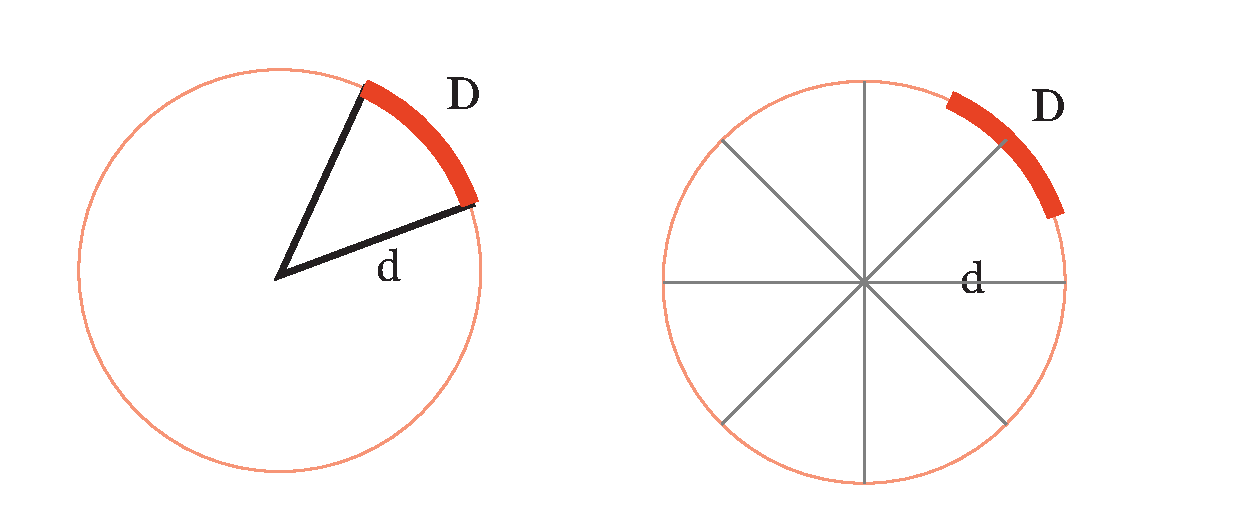
\includegraphics[width=0.8\textwidth, trim={0cm 0cm 0cm 0cm},clip]{Illustrations/Fig1_2.pdf}
  \caption{Left hand: $\hat{\gamma_c}$ : Classical share. Right panel: $\hat{\gamma_L} = \frac{1}{8}$ share}
      \label{fig:thepizza}
\end{figure}

\subsection{The Lightlane Equality }
In the limit, these two equations are equivalent. Recalling equation \ref{eq:classicalPC}, let $\theta_D$ be the angle occupied by the detector. The expected number of lightlanes that a detector $D$ intersect with is given by the angle it occupies divided by the angle between lightlanes.

\begin{equation}
\hat{L} =   \frac{\theta_D }{ 2\pi 2^b } \quad\quad 	L \in \mathbb{R},b \in \mathbb{Z}
\label{eq:hatL}
\end{equation}

For the right panel, the light emitted is constrained to travel in $2^b$ lightlanes. This means that the expected number of photons per lightlane must be given by $\hat{E_L}$
\begin{equation}
 \hat{E_L} = \frac{E}{2^b}, \quad\quad	\hat{E_L} \in \mathbb{R}, \quad E, b \in \mathbb{Z}
 \label{eq:expectedPhotonsPerLane}
\end{equation}

We now have expected number of lightlanes $\hat{E}_L$ intersected by Detector $\theta_D$,  and expected number of lanes that our detector is intersecting with  $\hat{L}$. The expected total number of Photons on detector then becomes.
\begin{equation}\label{eq:TauXdefinitionShort}
\gamma_L =  \hat{L} \hat{E_L} 
\end{equation}

Substituting $\hat{E_L}$ and $\hat{L} $ with equations, and simplifying give us.
\begin{equation}
 \gamma_L = \frac{2^b \theta_D}{2\pi} \frac{E}{2^b} = \frac{2^b \theta_D E}{2^b2\pi} =  \frac{ \theta_D}{2 \pi} E 
 \label{eq:Lightlaneequality}
\end{equation}

Compare equations for $\hat{\gamma_c} $ and $\hat{\gamma_L} $ and notice how equation  \eqref{eq:Lightlaneequality} and  \eqref{eq:classicalPC} are equal. On the surface, this is a trivial result of quantizing and then de-quantizing using the continous limit. But this has a possible interpretation that is quite profound. If the expected value is exactly the same in both a infinite directional movement and in the Lightlane variant taking into account the amount of directional information the photon carries with it, the classical equation  $\hat{\gamma_c} $ could well be an approximation for $\hat{\gamma_L} $, assuming sufficiently high bitlength.


\subsection{Concepts : Dark zones and Lucky Lanes}
However, there is an important difference between  $ \gamma_L $ \eqref{eq:TauXdefinitionShort} and $ \gamma_c$ \eqref{eq:classicalPC}  which comes into play as we vary the position of the emitter and detector.
While keeping in mind that  $\gamma_L$  and $ \gamma_c$ have the exact same Expected value( because the term $2^b$ disappears from the equation through simplification), this term isn't always irrelevant. In Figure \ref{fig:SmallDetector} we can see this in action : A tiny detector capturing an full $\frac{1}{8} $ of available photons, despite its musch smaller share of the circumference. We call this the "Lucky Lane effect". Clearly, the left hand in Figure \ref{fig:SmallDetector}is overperforming and the right hand is underperforming given the classically expected value $\gamma_c$. The difference between $\gamma_c$ and $\gamma_{Lc}$ is therefore affecting the variance. 
\begin{figure}[!ht]
  \centering

 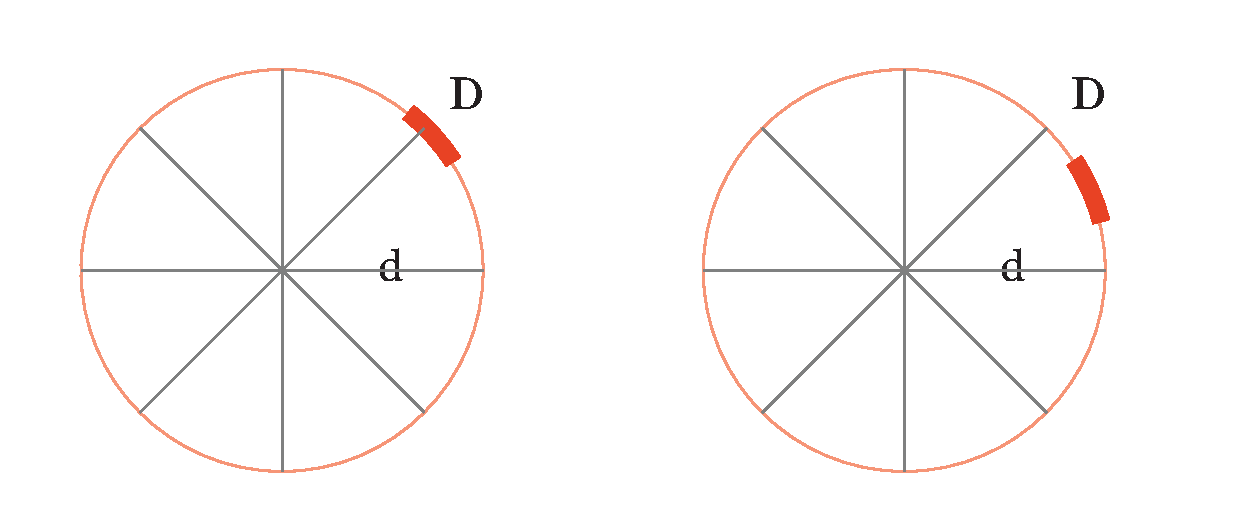
\includegraphics[width=0.8\textwidth, trim={0cm 0cm 0cm 0cm},clip]{Illustrations/Fig2.pdf}
  \caption{Left hand side : Detector is considerably smaller, but still, obtaining $\frac{1}{8} $ of photons emitted. Right hand side : Detector is in dark zone, receives no photons }
    \label{fig:SmallDetector}
\end{figure}

As shown to the left panel in Figure \ref{fig:SmallDetector}, a carefully positioned detector with $ \theta_D < \frac{2 \pi}{ 2^b} $ can receive $\hat{E}$ photons emitted, provided that the relative position remain fixed. In the right panel, the opposite case where   (Figure \ref{fig:SmallDetector}, right panel) illustrates that number of photons received can be either zero, or exactly $\frac{E}{2^b}$.  This is very different from the Expected Photon count $\hat{\gamma_c}$. This special edge-case is called a dark-zoned detector, charaterized by equation \ref{eq:darkZoneEquation}.

\begin{equation}
 \gamma_{L} = 0  \neq \hat{\gamma_L}
 \label{eq:darkZoneEquation}
\end{equation}

In a more general sense, the detector can either intersect with $L$ lightlanes or $L+1$. No other options are permissible (in 2D). These are called the low $L$ and the high $L +1$ lanecount respectively. If the detector $\theta_D > \frac{2\pi}{2^b}$, it can never be darkzoned - but it can alternate between the low number of lightlanes $L$ and the high number $L+1$, provided it is moving.

\subsection{Moving detectors - The Twinkle Density}
In Figure \ref{fig:MovingDetector} the detector  moving at a steady pace around the circumference. This ensures that it will receive both the low lanecount $L$ and the high lanecount $L+1$ as it orbits the emitting point. In the right panel of Figure \ref{fig:MovingDetector}, the detector has passed through several dark zones (green) where $L = 0$ and several lightlanes $L =1$, during a time interval $s$. 

It follows quite nicely from this that the decimal part of $\hat{\gamma_L}$ must correspond to the proportion of  time that the detector intersect an \textbf{additional} lane or not (however, this gets more complex in higher dimensions, see \cite{RhadamantysA3}). 

\begin{figure}[!ht]
  \centering

 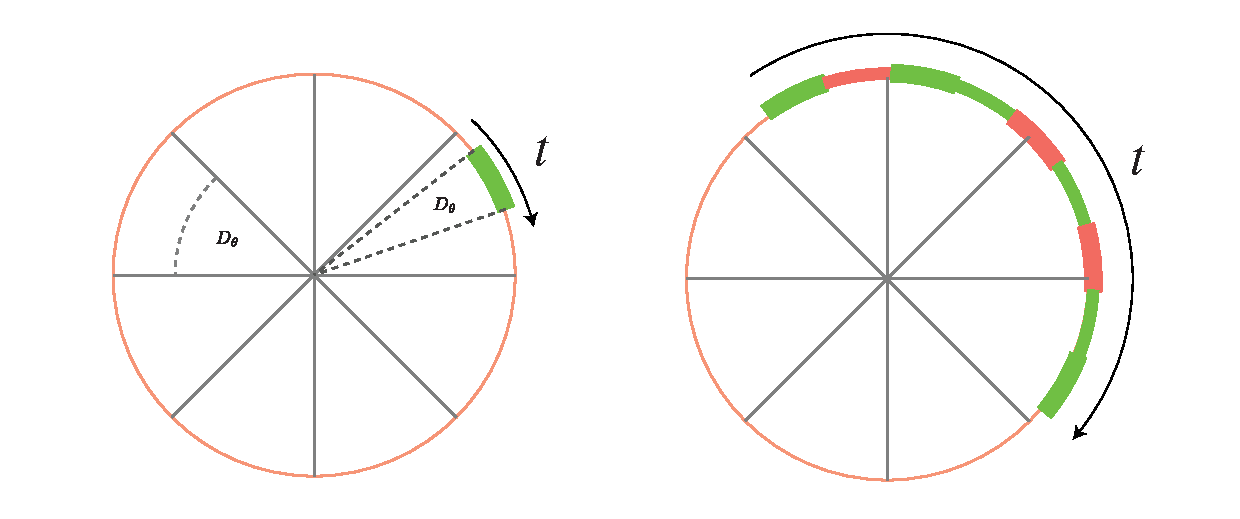
\includegraphics[width=0.8\textwidth, trim={0cm 0cm 0cm 0cm},clip]{Illustrations/Twinkle.pdf}
  \caption{Moving detector will either intersect with N lightlanes, or with N+1 lightlanes. }
    \label{fig:MovingDetector}
\end{figure}

Let us imagine expected lane count ($ \hat{L} $) is equal 2.54. This can then be interpreted as intersecting three lanes $54\%$ of the time, and two lanes $46\%$ of the time. This allows us to compute the expected photon count $\hat{\gamma_L}$ for the Lightlane setup as a class probability distribution called Twinkle densities:

\begin{definition}{\large Twinkle density (2D)} 
Let $L$ be the lowest number of intersections, and $p$ be the probability of intersecting with $L$ lanes. The number of lightlanes intersected is given by the density function. 
\begin{equation}
\label{eq:TwinkleDensity2D1}
L =
\begin{pmatrix}
pL \\
(1-p)(L+1)\\
\end{pmatrix}
\quad	L \in \mathbb{Z}, \quad p \in [0, 1] \cup  \mathbb{R}
\end{equation}
\end{definition}

It follows that the expected value for the number of lanes is given by:
\begin{equation}
\label{eq:TwinkleDensity2D2}
\hat{L} 
=
pL + (1-p)(L+1)
\in \mathbb{R}
\end{equation}


As the number of photons received are given by the lanecount multiplied by the emitted photons $E$ distributed over accessible lanes $2^b$, we can define:

\begin{definition}{\large Expected photon count  equation (2D)} 
Let $\hat{L}$ be the expected value for number of lightlanes intersected by the detector. The expected value of photons received $\hat{\gamma_L}$ will then be given by:
\begin{equation}
\label{eq:gammaL}
\hat{\gamma_L} =
\frac{E}{2^b}
\hat{L}
\end{equation}
\end{definition}

 The Twinkle is a proper density function, for example the (2D) Twinkle for $\hat{\gamma_{L}} = 2.54$ will be $N = 2, p = 0.46$. In the simple case where the detector orbits the source, both $ \theta_D $ and $d$ remains the same during the entire photon collection, the probabilities do not change over time. This means the photon timeseries distribution can be explained from knowing a Twinkle density along with a periodicity. 
 
This could, at least in theory, be detectable as fluctuations. These details will be investigated further in \cite{RhadamantysA3}. It is also possible to reverse engineer Twinkles, working backwards from observed variance in received photons over time. For example, if observed flux falls by exactly 33.3333\% from the peak periodically, we are likely to be observing a $L=2$ twinkle (in 2D). The probabilities simply determine how much time we are observing 2 vs 3 lightlanes.

\subsection{Lightlane Equality of the mean}
When $\lim_{b \rightarrow \infty}$ , $\hat{L}$ must also increase to infinity because:
\begin{equation}
\lim_{b \rightarrow \infty} \hat{L} = \theta_D \left( p (\frac{2^b}{2 \pi}) + (1-p)(\frac{2^b}{2\pi}+1)\right)
\approx \theta_D \frac{2^b}{2\pi}
\end{equation}

If we plug in this limit for $\hat{L}$ into the expected photon count equation, we simply reverse the quantization of directional freedom. Then we see that the classical and quantized versions agree:

\begin{equation}
\hat{\gamma_L} = \frac{E}{2^b} (\theta_D \frac{2^b}{2\pi})  = E \frac{\theta_D}{2\pi}  = \hat{\gamma_c}
\end{equation}

This equality of the mean requires a sufficiently high value for $b$ so that the difference between $L$ and $L+1$ lanes are neglible. However, it is important to note that this can also happen for lower values of $b$, provided that the detector is moving, and that the period available for collection $s$ is long enough for the detector to pass in and out of several lightlanes. This results in an effect where the value of $\hat{L}$ are a time average of $pL + (1-p)(L+1$) as in figure  \ref{fig:MovingDetector}, (right panel). This allow us to formulate a theorem:

\begin{theorem}[Lightlane Equality]
The expected photon count $\gamma_c$ for a classical (directionally unconstrained) point emitter equals that of directionally constrained emitter $\gamma_{L}$, if their relative velocity is not 0, or the bitlength is high enough to crowd out the effect of the additional lane. 
\end{theorem}

The result is generalizible to higher higher dimensions and other geometries than the point emitter, but it will get somewhat more complex because there are more than two alternating states, which also depend on the cross section geometry of the detector and the emitter. This will be addressed in the next paper called General Theory of Lightlanes \cite{RhadamantysA3}. 

\section{Variance}
We will now explore the effect on the variance. Variance is defined as \textbf{the expected value of the square of the deviation from the mean}. Intuitively, we see that we can reduce the effect of the time-averaging by using a shorter capture time $s$, leaving only the first averaging mechanism. If we also lower the bitlength $b$, we will eventually reduce the expected lane-count number $\hat{L}$ until it is no longer possible to realize the exact values for $p$ which would guarantee the Lightlane equality to hold $\hat{\gamma_c} = \hat{\gamma_L}$. Consider for example, if the lanecount is $\hat{L} = 1.4$ and the shutter time is infinitesimally short. Then, we will for each frame, have a $60\%$ chance of receiving from exactly one lane, and a $40\%$ chance of receiving from exactly two lanes. Also, we should expect that the next frame have the reverse proportion. This effect rapidly declines with increasing shutter time $s$ and higher lanecounts because both effect contribute to realizing the Lightlane Equality. 

In the following we will show an example, and estimate the maximum and minimum size of this discrete deviance as a function of lanecount. We recall from equation \eqref{eq:hatL} that expected lanecount is itself a function of bitlength $b$, the size of the detector $\theta_D$ and the distance from the emitter $d$.
\begin{equation}
\hat{L} = f(\theta_D, b) = \frac{\theta_D }{ 2\pi 2^b } \quad\quad 	b \in \mathbb{R}
\end{equation}

 Intuitively we know that the deviance will be fluctuating on both sides of the mean, corresponding to the low lanecount or the high lanecount component being stronger for a particular capture frame. 
 
 We recall that expected Photon count for Lightlane is given by.
 \begin{equation}
\label{eq:Twinkle1_repeated}
\hat{\gamma_L} =
\frac{E}{2^b}
\hat{L}
\end{equation}

The variance component associated with Lightlane Equality violation must then be :
\begin{equation}
\label{eq:VarianceDefinition}
\sigma_L^2 = \left( \gamma_{L}- \gamma_c \right)^2 
\end{equation}
We will unpack this definition for the Variance, for reference see \eqref{eq:TwinkleVariance1} for $\gamma_L$ and \eqref{eq:classicalPC} for $\gamma_c$. The variance is more sensitive to the underlying discrete complexity than the mean. If anomalous patterns are detected in the mean, then the variance should also follow a related pattern which we will now define. Let the Twinkle density under consideration be that from \eqref{eq:Twinkle1_repeated}, toggling between a low $(L=2)$ and a high $(L=3)$ lanecount with $p = 0.54$. As the detector moves, the lanecount toggles between $2$ and $3$ lanes realizing a mean of $\hat{L} = 2.54$. We insert these values into the variance:

\begin{equation}
	\sigma_L^2 = \left( E\left(0.54 \cdot (\frac{3}{2^b}) + 0.46 \cdot (\frac{2 }{2^b}) \right) - \gamma_c \right)^2
	\label{eq:TwinkleVariance1}
\end{equation}

We immediately see the symmetry inside inner parenthesis, indicating that as long as the probabilities realized during the shutter window $s$ are exactly $0.54$ and $0.46$, the two terms perfectly cancel out, resulting in a Lightlane variance contribution of 0. However, this depends on the conditions mentioned above: Either sufficiently high values for $L$ or sufficiently long capture window $s$ or both. A longer $s$ acts to time-average the high and low lanecount components, realizing the two required values for $p$ to make the lightlane variance component go away. However, it is clear that for a short enough shutter time $s$, the detector can be either in the low or the high lanecount for the entire duration of $s$. This would yield observed values for $p$ that deviate from those required to produce the internal cancellation. Consequently, unexplained observed variance could be explained by the realized value of $p$ - named $p_r$ - is deviating from the value of $p$ associated with internal cancellation.

Before we proceed, make sure you understand the past example. (If you don't, it will be hard to understand the motivation for the following). 

\subsection{Generalized Lightlane variance in 2D}
Consider a moving telescope observing incoming photons from a distant star, for a period of time $s$, and accept for a moment that we are operating in two dimensions only. We would like to produce a contribution to the variance caused by Lightlane Equality violation. We will first generalize the above equation \eqref{eq:TwinkleVariance1} using the values $p$, $\gamma_L$ as well as $L$ and $L+1$ for the low and high lanecount, and use the realized value $p_r$ for a capture frame of duration $s$. 

\begin{equation}
	\sigma_L^2 = \left(E\left(p_r \cdot (\frac{L+1}{2^b}) + (1-p_r) \cdot (\frac{ L }{2^b}) \right)- \gamma_c \right)^2
	\label{eq:TwinkleVariance2}
\end{equation}

The amount of possible deviance of $p_r$ relative to $p$ is a function of the angle between lightlanes $\frac{2\pi}{2^b}$, the size of the detector $\theta_D$ and the area covered by the detector during the time $s$. Let $s = 1 ms$, and the speed (in radians) of the detector be $\theta_v$ per millisecond. The detector now covers an area of $\theta_D + \theta_v$.

The remainder between the capture area of the detector and the angle between individual lightlanes, represents the asymmetry of the realized exposure to the low and high lanecount components. Suppose for example, that the during the capture window $s$, the detector passes through 3.34 lightlanes. This means it must either:

\begin{enumerate}
\item Lower bound : Pass through 2 low lanes and 1.34 high lanes.
\item Upper bound : Pass through 1.34 low lane and 2 high lanes
\end{enumerate}

We can use these to compute the maximum and minimum realizable values for $p_r$, which we denote $\underline{p_r}$ and $\overline{p_r}$. It is clear that we are passing fully through 3 lanes. However, we require the remainder $m$, which should be equal to 0.34 in this example. The meaning of this $m = 0.34$ is that the detector has entered into the fourth lane $(n+1 = 4$), and at the time where the shutter time ends, it has been exposed to 34\% of the $(n+1)th$ lane. 

\begin{equation}
m =  \left(\theta_D + \theta_v  \right) \mod \frac{2\pi}{2^b}
\end{equation}

We also need the principal $n$, which we get through integer division (in this case it becomes 3).

\begin{equation}
n =  \left(\theta_D + \theta_v  \right) / \frac{2\pi}{2^b}
\end{equation}

This gives us half the number of lightlanes we have passed through, rounded down - plus the remainder. 
\begin{equation}
\underline{p_1} = n / 2, \quad \underline{p_2}		 = 	n- n/2 + m
\end{equation}

For the upper bound, we get:

\begin{equation}
\overline{p_1} = n- n/2 + m \quad \overline{p_2}		 = 	n/2
\end{equation}

Inserting for $\overline{p}$ and $\underline{p}$ into $\hat{\gamma_L}$, and then expanding $\hat{\gamma_L}$ in the equation for variance \eqref{eq:VarianceDefinition}, we get two equations for variance, corresponding to maximum underestimation and overestimation errors. These represent boundaries for how much additional variance can be caused for a given bitlength. 

\begin{equation}
\underline{\sigma_L^2} 
 = \left(E\left((n / 2)  \cdot \frac{((L+1)}{2^b})
  + (n - n/2   +m) \cdot \frac{( L )}{2^b} \right) - \hat{\gamma_c} \right)^2
	\label{eq:TwinkleVariance3}
\end{equation}
\begin{equation}
\overline{\sigma_L^2}
	 = \left(E\left(n-(n / 2) + m) \cdot \frac{((L+1))}{2^b} + (n/2   ) \cdot \frac{( L )}{2^b} \right)- \hat{\gamma_c} \right)^2
	\label{eq:TwinkleVariance4}
\end{equation}



\subsection{Possible application of the variance equations}
If we successfully convert these equations into 3D, we obtain a new component to variance by parametrizing. There are many issues to be addressed, for example, we have not yet taken into account the size and shape of the emitting object, and our requirements for the velocity vector of the detector is simplistic. Such difficulties aside, the theory points to possible tests that can be done on datasets from Telescopes.

\begin{enumerate}
\item \textbf{Next frame tests} : It follows from the theory that the  variance will fluctuate between the over and underestimation extremes in a period way. 
\item \textbf{Unexplained variance} can be parametrized using $L$ and $p_r$ within the constraints, and fitted to the datasets.
\item \textbf{Fluctuations in moving average} can be used to extend the boundaries for $p_r$, giving greater room for fitting.
\end{enumerate}

\section{Conclusion}
The Lightlane Conjecture is the first foray into exploring the consequences of constrained directional freedom for photons, imposed by postulating Cellular Automaton models of the photon, propagating on a quantized substrate. 
Assuming an universal grid and that Cellular Automata constraints are relevant to photons, we constrain the directional freedom of photons. Constructor Theory acts a theoretical foundation for interrogating what information system can and cannot possibly do. This enables a way to make contact between deterministic, grid-based Quantum Foundation theories that rely on compatible assumptions, possibly falsifying entire of Celluar Automata. This can be done by conclusively proving that light is not constrained by carrying information about it's propagation path. Perhaps this paper can inspire others to take similar approaches to other quantum phenomena on which Cellular Automata constraints can be refined into empirical tests. 

The only empirical result of this paper is if light has directional freedom (EDI) in excess of $EDI > 2^{b-1}, \quad b >= 204$, the directional resolution is so high that it remains completely indistinguishable from the classical, continuous equations which assume infinite directional freedom, even for a much more advanced civilization than ourselves. However, if the bitlength is much lower, it might be possible to make predictions about photonic behaviour that is inconsistent with current formulations of any established physical theory that implicitly assume infinite directional freedom. Specifically there might be detectable real world phenomena in short-capture frame Telescope data from distant stars, by contributing a variance component to the flux. Detecting this component will allow breaking the Lightlane equality. Another important find is that the \textbf{variance} is more sensitive than the mean, and their respective relation to each other follows from the parametrization, giving opportunity for a two sided test. We, that is I, welcome anyone out there, professional or amateur to look into data from telescopes to prove this theory is wrong.

\begin{appendices}
In this appendix we introduce some metrics for TCAs which are not used in the paper, but might be of some interest. 
\section{Classifying CAs}


For the Glider pattern, we notice that the pattern will loop back to state 1 from state 4, but with a displacement. We define the displacement $\vec{d}$,  the periodicity $P =4$ and the velocity $\vec{v}$.

\begin{equation}
\vec{d} = \begin{pmatrix}
x \\ y 
\end{pmatrix} = 
\begin{pmatrix}
1 \\ -1 
\end{pmatrix}, \quad \vec{v}= \frac{ \vec{d}}{P}= \begin{pmatrix}
\frac{1}{4} \\ -\frac{1}{4} 
\end{pmatrix}
\end{equation}

In a simlar way to eigenvectors being embedded within a matrix, the vector $\vec{d}$ and periodicity $P$ is embedded in the relationship between the Game of Life rules, and the initial conditions. By rotating the initial conditions in the first frame, we can see how we can realize four distinct propagation directions. Other directions are not possible. There exist many other CAs with other displacement vectors embedded. Through Shannons source coding theorem, we know that the amount of information \textit{embedded} in the CA cannot exceed the total amount of information in the CA. \cite{shannon1}. Therefore, an assumption that a CA is assumed to have infinite directional freedom, it must also have infinite information. It is possible that CAs are large, and can possibly carry a very large amount of information about its direction through space. This converts the problem from an infinite to a finite problem.

The mechanism is a-priori deterministic and periodic. The Glider in Figure \ref{fig:glider} serves as an excellent mental placeholder symbol. But it's important to remember that TCAs are an extremely large subgroup of information and complexity theory, and that different rules produces different TCAs in different crystal lattices. Therefore it is meaningful to talk about features that are shared across all TCA:

\begin{enumerate}
\item Periodicity : $P$ The number of iteration before looping
\item Velocity : $\vec{v}$ The average displacement per iteration
\item Displacement : $\vec{d}$ The displacement per P iterations.
\end{enumerate}

\subsection{Planck-time subdivision}
Quantum mechanics suggest that the smallest possible time increment is the Planck Length. This metric is connected to the speed of light, and the Planck length. In order to make CAs travel at the speed of light, they must be able to move one tile for each unit of planck time along the euclidian distance metric. However, there is nothing to stop us from subidiving time further, provided this is the maximal speed. We would like to create a time unit called operations, which is an integer subdivision of planck time. 

\begin{definition}
\textbf{ \textit{Operations} \textbf{(o)}}: An operation  is a deterministic tranformation of the pattern into another form, following a rule. The count of such operations $o$ is used as a time metric, where $|\vec{v}|_M$ is the Manhattan distance metric of the displacement vector, $o$ is the time.
\begin{equation}
|\vec{v}|_M \leq o
\end{equation} 

Each \textbf{op} is an integer fraction of Planck time $T_P$, and  $\Omega$ the integer scalar.
 
\begin{equation}
\frac{T_P}{\Omega} = o, \quad \Omega \in \mathbb{Z}^+
\end{equation} 
\end{definition}

Like in quantum mechanics, information cannot be between spacetime tiles, which are units of the Planck length.  The effect is that the euclidian distance metric becomes nonsensical. We can use the Weyl distance metric, and for $\mathbb{Z}^2$ this is the Manhattan distance.

\begin{definition}
\textbf{ \textit{Vector length} \textbf{($\vec{v}$)}}

The norm of a Manhattan distance  metric $|\vec{x}|_M $ is different from the Euclidian $|\vec{x}|$, and is the sum of the the directional components.
\begin{equation}
|\vec{v}|_M = v_x + v_y +... + v_n \neq \vec{v}_E = \sqrt{v_x^2 +v_y^2 +... + v_z^2}
\end{equation}
\end{definition}

\subsection{Classifying features of Cellular Automata}

In addition 


\begin{definition}
\textbf{\textit{Periodicity} \textbf{(P)}}:The number of operations before the pattern loops, i.e returns to a previous configuration (possibly at a different location). 
\end{definition}

\begin{definition}
\textbf{\textit{Displacement (per loop)} \textbf{($\vec{x}$)}}: The change in the position of TCA after completing a loop
\begin{equation}
\vec{x} = \vec{x_{o+P}} - \vec{x_o}
\end{equation} 
\end{definition}



\begin{definition}
\textbf{\textit{Velocity}  \textbf{($\vec{v_M}, v_M$)}}:The average amount of displacement executed per unit of Planck time, using the Manhattan distance metric.
\begin{equation}
\begin{split}
v_M = |\vec{v_M}|
\end{split}
\end{equation} 
\end{definition}

\begin{definition}
\textbf{\textit{Footprint} \textbf{($ F $)}}: The maximum number of cells occupied by information belonging to the Cellular Automaton in a cycle.
\end{definition}

\subsubsection{Glider characteristics}
This allows us to compute the values for the Glider in Conways Game of Life:
\begin{center}

\begin{tabular}{ c c c }
\hline
 Property & Symbol & Glider Value \\ [0.5ex]
 Effective Directional Information & EDI & 4 \\ 
 Bitlength & b & 2 \\ 
 Periodicity & P & 4 \\  
 Displacement per loop  & $\vec{x}$ & $(\pm 1, \pm 1)$    \\
 Velocity (vector) & $\vec{v}$ & $(\pm \frac{1}{4} ,\pm \frac{1}{4})$    \\
 Velocity (scalar) & $\vec{v}_M$  & = $\frac{1}{2}$ \\
 Planck time conversion & $\Omega^{-1} $ & 2\\
 Footprint 	& F & 5
\end{tabular}

\end{center}
\end{appendices}
\bibliographystyle{plain}
\bibliography{../mybib}


%\includegraphics[width=0.65\textwidth]{eps_demo}
\end{document}
